\subsubsection{Lógica de control modo limitado e intermitente}


El SAL/T cuenta con dos modos donde las señales críticas de corte de tracción y freno de emergencia son activadas y liberadas de manera dinámica; en el modo aislado limitado y en el modo intermitente. El modo aislado limitado se activa de manera local con la llave rotativa ubicada en el panel frontal del SAL/T; en este modo se utilizan las mediciones de velocidad y ubicación para determinar la activación o liberación de las señales críticas. En caso de no contar con referencias de velocidad, se pasa automáticamente al modo intermitente (también accesible de manera directa mediante comando remoto desde la central operativa); en este modo, no se consideran la velocidad de circulación sino los tiempos configurados para la activación de las señales. Si al momento de activación del modo aislado limitado no se cuenta con referencia de velocidad, se activa el corte de tracción y freno de emergencia por 30 segundos.\\ 


En el modo aislado total existen cuatro perfiles de velocidades; el primero corresponde al perfil activado cuando no existe referencia de la ubicación de la formación y por lo tanto no se puede determinar la zona de circulación, los otros tres corresponden a las tres zonas de circulación definidas para el recorrido de la formación. Cada perfil cuenta con sus propias velocidades configuradas. Los parámetros configurados en cada perfil corresponden a la velocidad a la cual se debe activar el corte de tracción para desacelerar, la velocidad a la cual se puede liberar la señal de corte de tracción para volver a acelerar, la velocidad límite para activar el freno de emergencia (debe ser superior a la velocidad de desaceleración ya que se activan ambas señales críticas juntos para detener la formación) y el tiempo mínimo que ambas señales deben mantenerse activas tras superar el último umbral hasta llegar a una velocidad de detención. \\ 

El SAL/T, en modo aislado limitado, va a estar constantemente monitoreando la ubicación para seleccionar el perfil que corresponda y midiendo la velocidad de circulación para determinar si es necesario activar o liberar alguna de las señales mencionadas anteriormente. Además, en este modo se activa el buzzer sonoro de manera intermitente y al exceder alguno de los umbrales configurados, se activa el buzzer de manera continua para indicar el sobrepaso del umbral. \\



El modo intermitente tiene cinco perfiles disponibles en el que cada uno de ellos cuenta con los parámetros de tiempo de aceleración, tiempo de desaceleración, cantidad de ciclos antes de frenar y tiempo de frenado. El sistema va a determinar el perfil a ejecutar acorde a lo que seleccione el maquinista con un botón ubicado en el panel frontal y su correspondiente indicación luminosa que le permite visualizar el perfil seleccionado en caso de activarse de manera local, o el perfil seleccionado en el comando remoto si se activó el modo desde la central operativa. La idea de tener distintos perfiles disponibles y configurables corresponde con que los tiempos para cada formación pueden ser distintos dependiendo el material rodante sobre el que se aplique, condiciones externas o incluso la zona de circulación del momento.\\

El SAL/T va a ejecutar estar rutina de aceleración (de T segundos) y desaceleración (de D segundos) N veces para luego activar el freno junto al corte de tracción por E segundos; luego recomienza la rutina desde el comienzo. En la figura \ref{fig:intermitente} se visualizan los ciclos del modo intermitente viendo como se espera que varíe la velocidad a lo largo del tiempo. 

\begin{figure}[H]
    \centering
    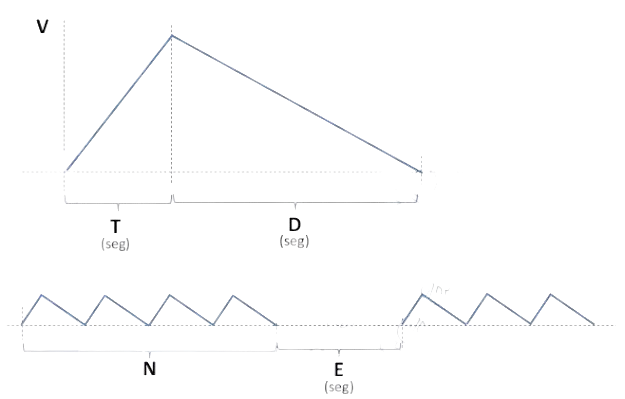
\includegraphics[width = \linewidth]{img/intermitente.png}    
    \caption{Perfil de velocidad de una formación en modo intermitente}
    \label{fig:intermitente}
\end{figure}    
